% !TeX root = OptCuts.tex

\section{Evaluation}
\label{sec:results}

\subsection{Implementation}
\label{sec:imp}

\minchen{
any important details of the libraries you used: triangle, libIGL
specs of the machine(s) used to time and evaluate methods:
3.1 GHz quad-core Intel Core i7
16 GB 2133 MHz LPDDR3
}

\minchen{Add energy plot to show convergence?}

\subsubsection{Initialization}
\minchen{merge initial embedding paragraph}
To obtain an initial UV map for an input surface, we map its initial seam to a circle preserving edge length and parameterize the rest of the vertices through Tutte embedding with uniform weights.

We compute initial seams for different surfaces according to their topology and geometry. For disk-topology surfaces, we simply pick their longest boundary as the initial seam. For genus-0 closed surfaces, we randomly pick 2 connected edges as the initial seam. \minchen{[TODO] change to curvest one point cut or farthest point cut if they are better} For high-genus surfaces, we follow Crane et al.~\shortcite{Crane:2013:DGP} to detect homology generators and connect all of them as the initial seam \minchen{[TODO]}.

We simply start by ignoring the distortion constraints with $\lambda$ set to $0$, and let our dual update to modify $\lambda$ according to the intermediate distortions.

\subsubsection{Continuous Search}
\label{sec:descentStep}

Our smooth descent steps take in the locally altered UV map by the current topology descent step and conduct one Newton-type iteration towards solving $\min_U E_d$ with $T$ fixed (Algorithm~\ref{alg:descentStep}).

\begin{algorithm}[h]
\SetAlgoLined
\KwData{$M$, $T^{k,i}$, $U_a^{k,i-1}$}
\KwResult{$U^{k,i}$, $\delta^{k,i}$}
$g^{k,i-1} \leftarrow \nabla E_{d}(T^{k,i}, U_a^{k,i-1})$\;
\If{$||g^{k,i-1}||^2 < 10^{-12}$}{
	converge\;
}
compute $E_{d}$ Hessian proxy $P^{k,i-1}$\;
solve $P^{k,i-1} p^{k,i-1} = -g^{k,i-1}$ for search direction $p^{k,i-1}$\;
compute initial step size $\alpha^{k,i-1}_0$\;
back-tracking line search with Armijo rule to obtain $\alpha^{k,i-1}$\;
$U^{k,i} \leftarrow U_a^{k,i-1} + \alpha^{k,i-1} p^{k,i-1}$\;
$\delta^{k,i} \leftarrow E_{d}(T^{k,i}, U^{k,i}) - E_{d}(T^{k,i}, U_a^{k,i-1})$\;
\If{$|\delta^{k,i}/E_{d}(T^{k,i}, U_a^{k,i-1})| < 10^{-6}\alpha^{k,i-1}$}{
	stop\;
}
\caption{Smooth Descent Step $(k+1,i)$}
\label{alg:descentStep}
\end{algorithm}
Since $E_{d}$ is not convex, we apply the projected Newton method\ \cite{Teran2005Robust} to project the Hessian of each energy element to its closest symmetric positive definite (SPD) matrix in parallel with Intel TBB~\cite{Reinders2007Intel}, and assemble them to form the SPD Hessian proxy $P$. We use the PARDISO~\cite{pardiso-6.0a, pardiso-6.0b} symmetric indefinite solver to solve the linear system $P p = -g$ for search direction $p$. \minchen{[TODO] change to use SPD solver by fixing a direction to ensure definiteness} As $E_{d}$ is also a barrier-type energy, it is essential to ensure that the configuration always stays inside the feasible region. Thus, we follow Smith and Schaefer~\shortcite{Smith2015Bijective} to first compute an initial step size $\alpha_0$ that avoids element inversion and then conduct back-tracking line search with Armijo rule~\cite{Armijo1966Minimization} to ensure sufficient energy decrease.

Besides a relatively small tolerance on $g$ for convergence detection, we apply another relative energy decrease criteria to appropriately stop the process while necessary.
This can stop our continuous search at the true local optimum infinitesimal better than setting a larger gradient tolerance since our energy is highly nonlinear.

\subsubsection{Global Bijectivity}
\label{sec:bijectivity}
Following Jiang et al.\ \shortcite{Jiang2017Simplicial}, we realize this additional constraint on our mapping by first triangulating the void regions of each iterations updated UV map using Triangle library\ \cite{Triangle_Engineering_a_2D_quality_mesh_generator_and_Delaunay_triangulator}. The void regions are consisted of all holes and the surrounding space of the UV map, bounded by its boundaries and a loose bounding box.
Then we augment our distortion energy $E_d$ with an additional term, \emph{not included in the distortion bound constraint}, to form a collapse preventing energy for the added negative-space triangles during each optimization iteration.

With this augmentation, our continuous search stays the same, while for our topology search, we need to also ensure that the negative-space triangles are added correctly when we query for our local topological operations.
Instead of re-using a loose bounding box, we take the current negative-space triangles into consideration when building up the local stencil near the edited seam. Since the boundary of the local stencils are all fixed during the query, this naturally prevent potential global overlaps with geodesically faraway UV elements. Similarly, the collapse preventing energy on the negative-space triangles is not involved in the computation of first-order reduction.
In splitting operations only, we also need to carefully push the splitted vertices in the opposite direction of their curvature normals before the querying optimization. This ensures that the initial local stencil has a collapse-free void region so that it could be triangulated correctly.

%\paragraph{Potential Accelerations for Practical Use}
%Since our topological operations only change the mesh locally both on connectivity and coordinates, we could also update the Hessian or the decomposition locally to save time. Besides, it is also interesting to try other Hessian approximation methods like L-BFGS~\cite{Liu1989Limited} or composite majorization~\cite{Shtengel2017Geometric} to explore further acceleration by finding a balance between per-iteration computational cost and convergence rate.
%\justin{not sure previous paragraph is needed}


\subsection{Method Evaluation}

We evaluate our method with/without global bijectivity by running them on 70 input surfaces including both disk-topology and closed surfaces (some are with \minchen{[TODO] high genus}), setting $b_d$ to $4.2$, $4.1$, and $4.05$ (Table~\ref{tb:stats_OptCuts}). Our methods automatically generate high quality UV maps given any distortion bounds for all inputs without any user assistance (Figure~\ref{fig:our_impressive_results}).

\begin{table}[!h]
\centering
\caption{Statistics of OptCuts running on 70 input surfaces with each of the 3 distortion bounds ($b_d = 4.2$, $4.1$, and $4.05$) both with and without bijectivity enabled.}
\label{tb:stats_OptCuts}
\begin{tabular}{|c|c|ccc|ccc|}
\hline
\multirow{2}{*}{$b_d$} & \multirow{2}{*}{bijectivity} & \multicolumn{3}{c|}{$E_{s}$} & \multicolumn{3}{c|}{time (s)} \\ \cline{3-8} 
                       &                         & avg      & min     & max      & avg       & min    & max      \\ \hline
\multirow{2}{*}{4.2}   & OFF                    & 3.819   & 0.080  & 14.545  & 87.0   & 0.3 & 417.8 \\
                       & ON                & 4.087   & 0.289  & 17.063  & 190.3   & 3.8 & 983.3  \\ \hline
\multirow{2}{*}{4.1}   & OFF                    & 4.709   & 0.752  & 17.980  & 137.5  & 0.9 & 886.9 \\
                       & ON                & 5.324   & 0.860  & 21.595  & 271.1   & 6.9 & 1767.8  \\ \hline
\multirow{2}{*}{4.05}  & OFF                    & 6.142   & 0.277  & 21.566  & 213.2  & 3.9 & 1398.1   \\
                       & ON                & 7.195   & 0.932  & 29.596  & 412.9   & 7.2 & 2859.5 \\ \hline
\end{tabular}
\end{table}

\begin{figure*}[!h]
\centering
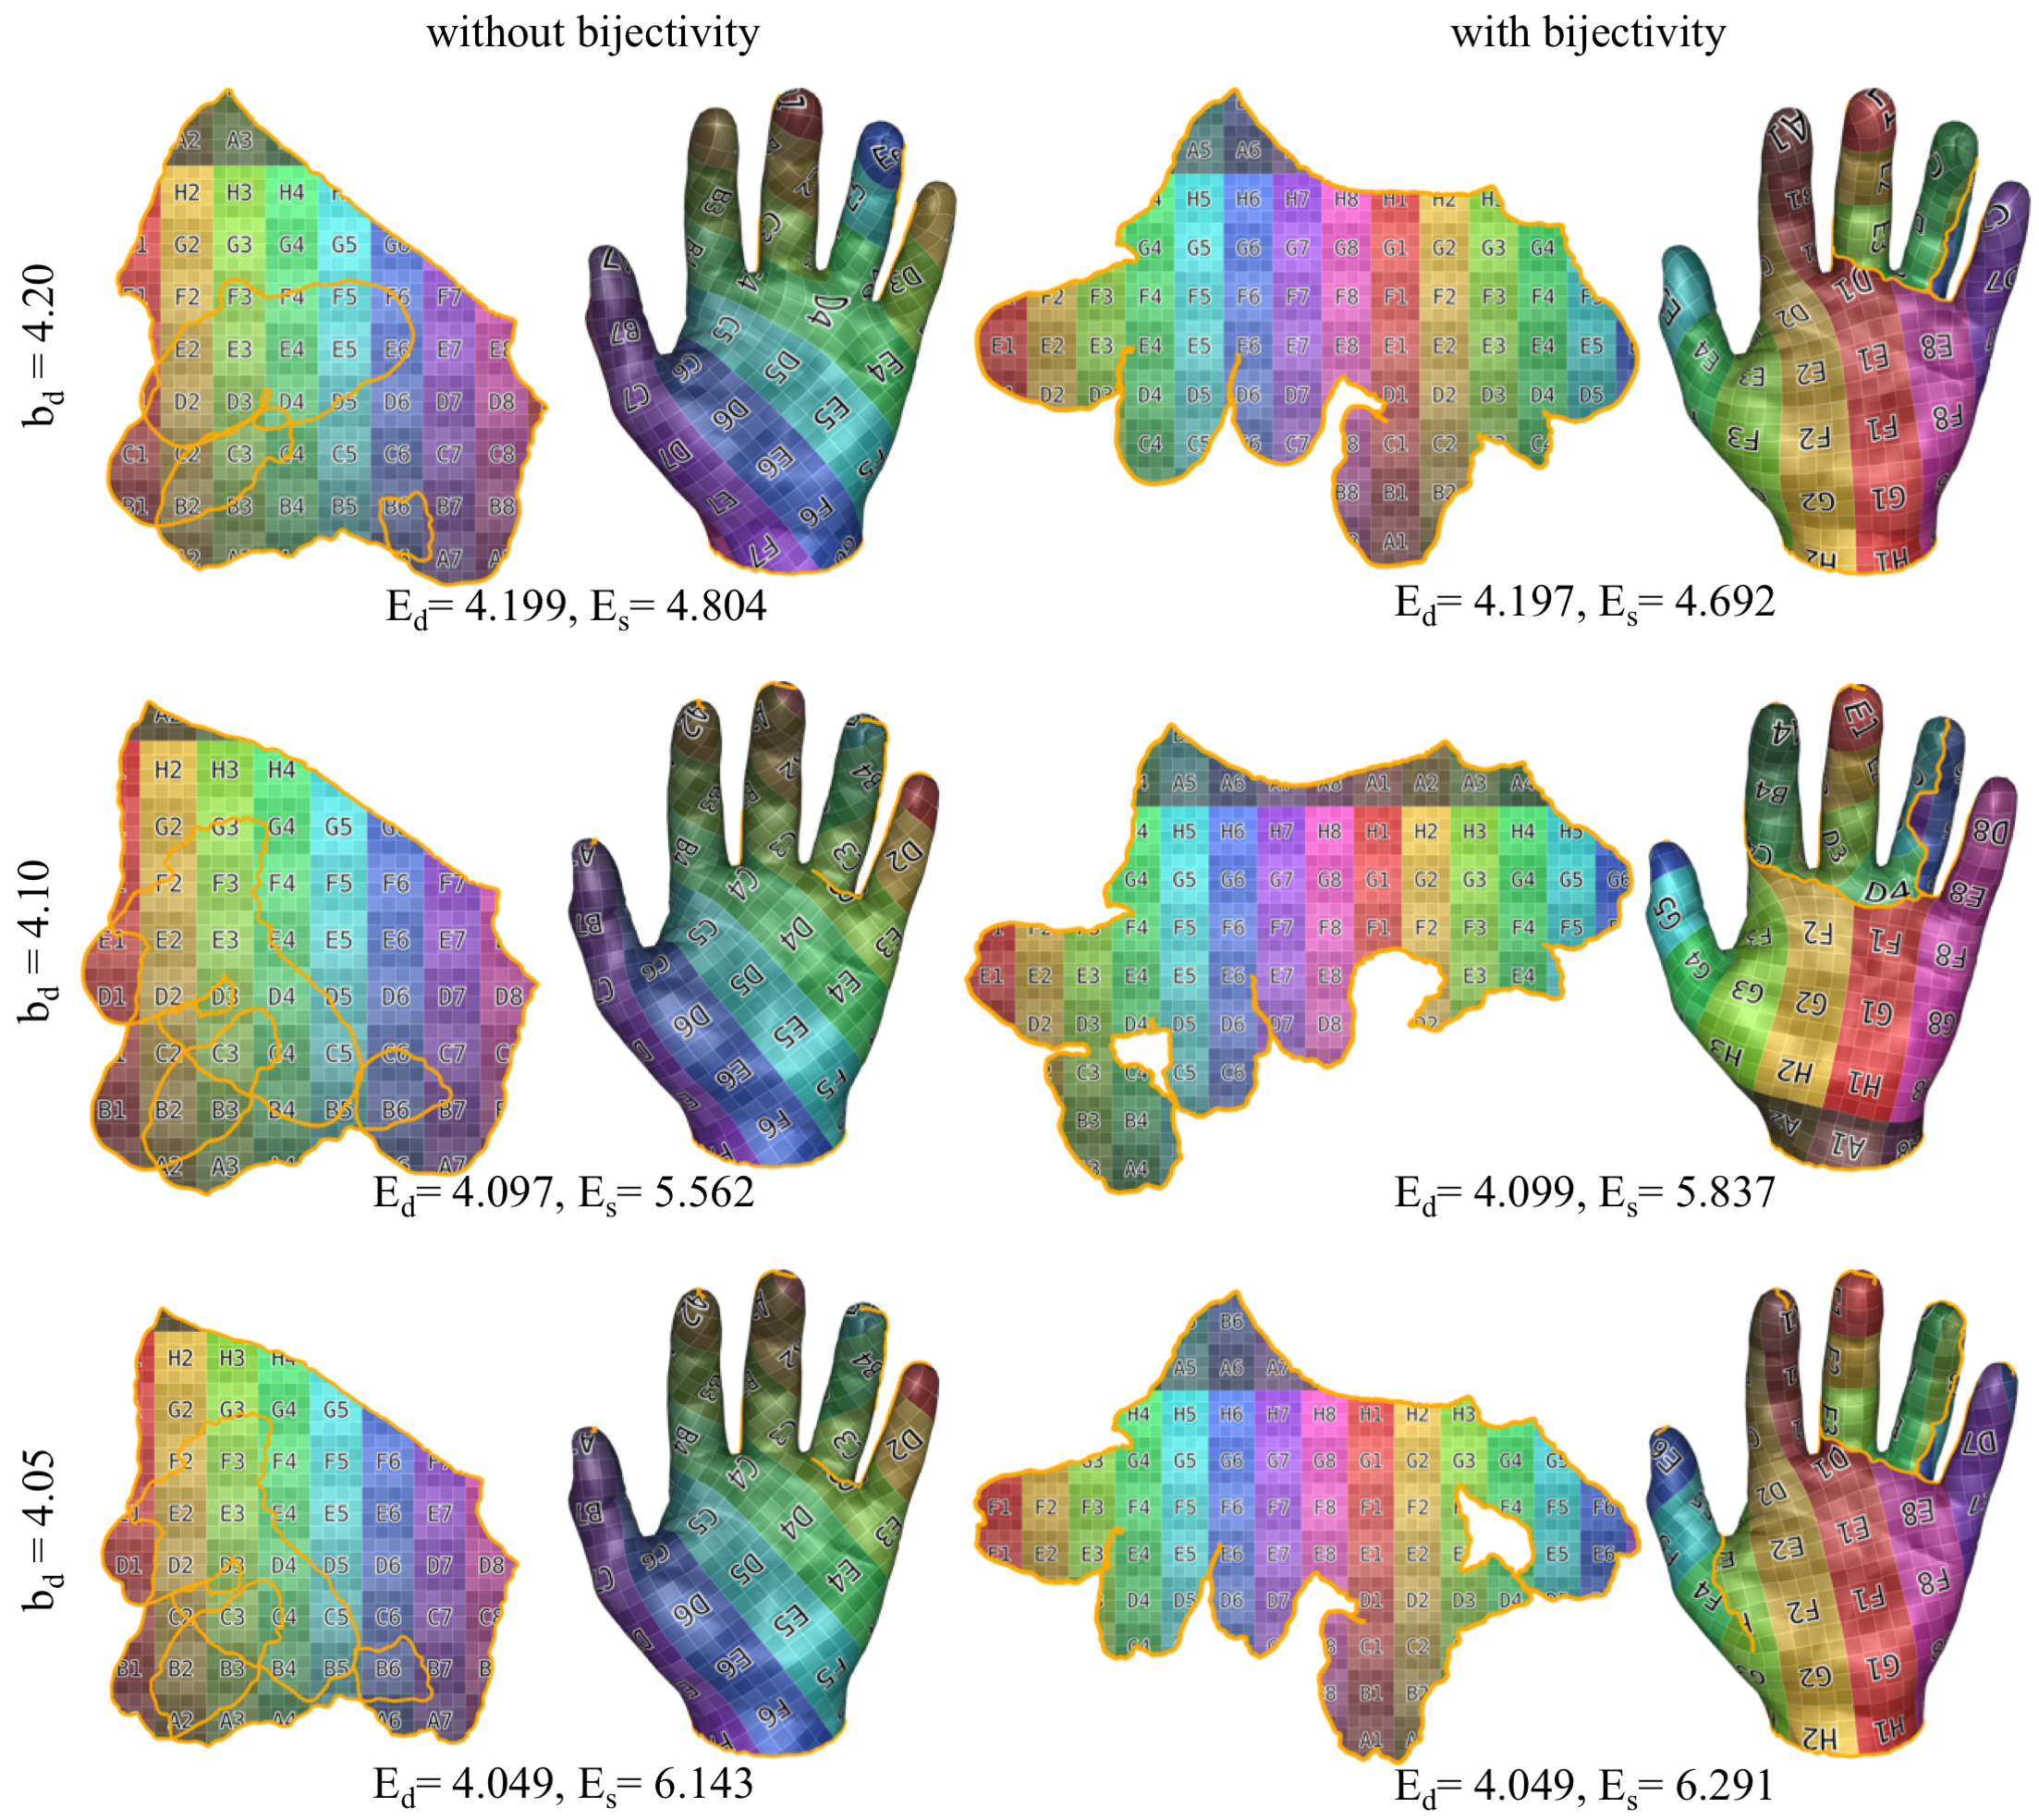
\includegraphics[width=0.48\linewidth]{fig/our_impressive_results_left.png}
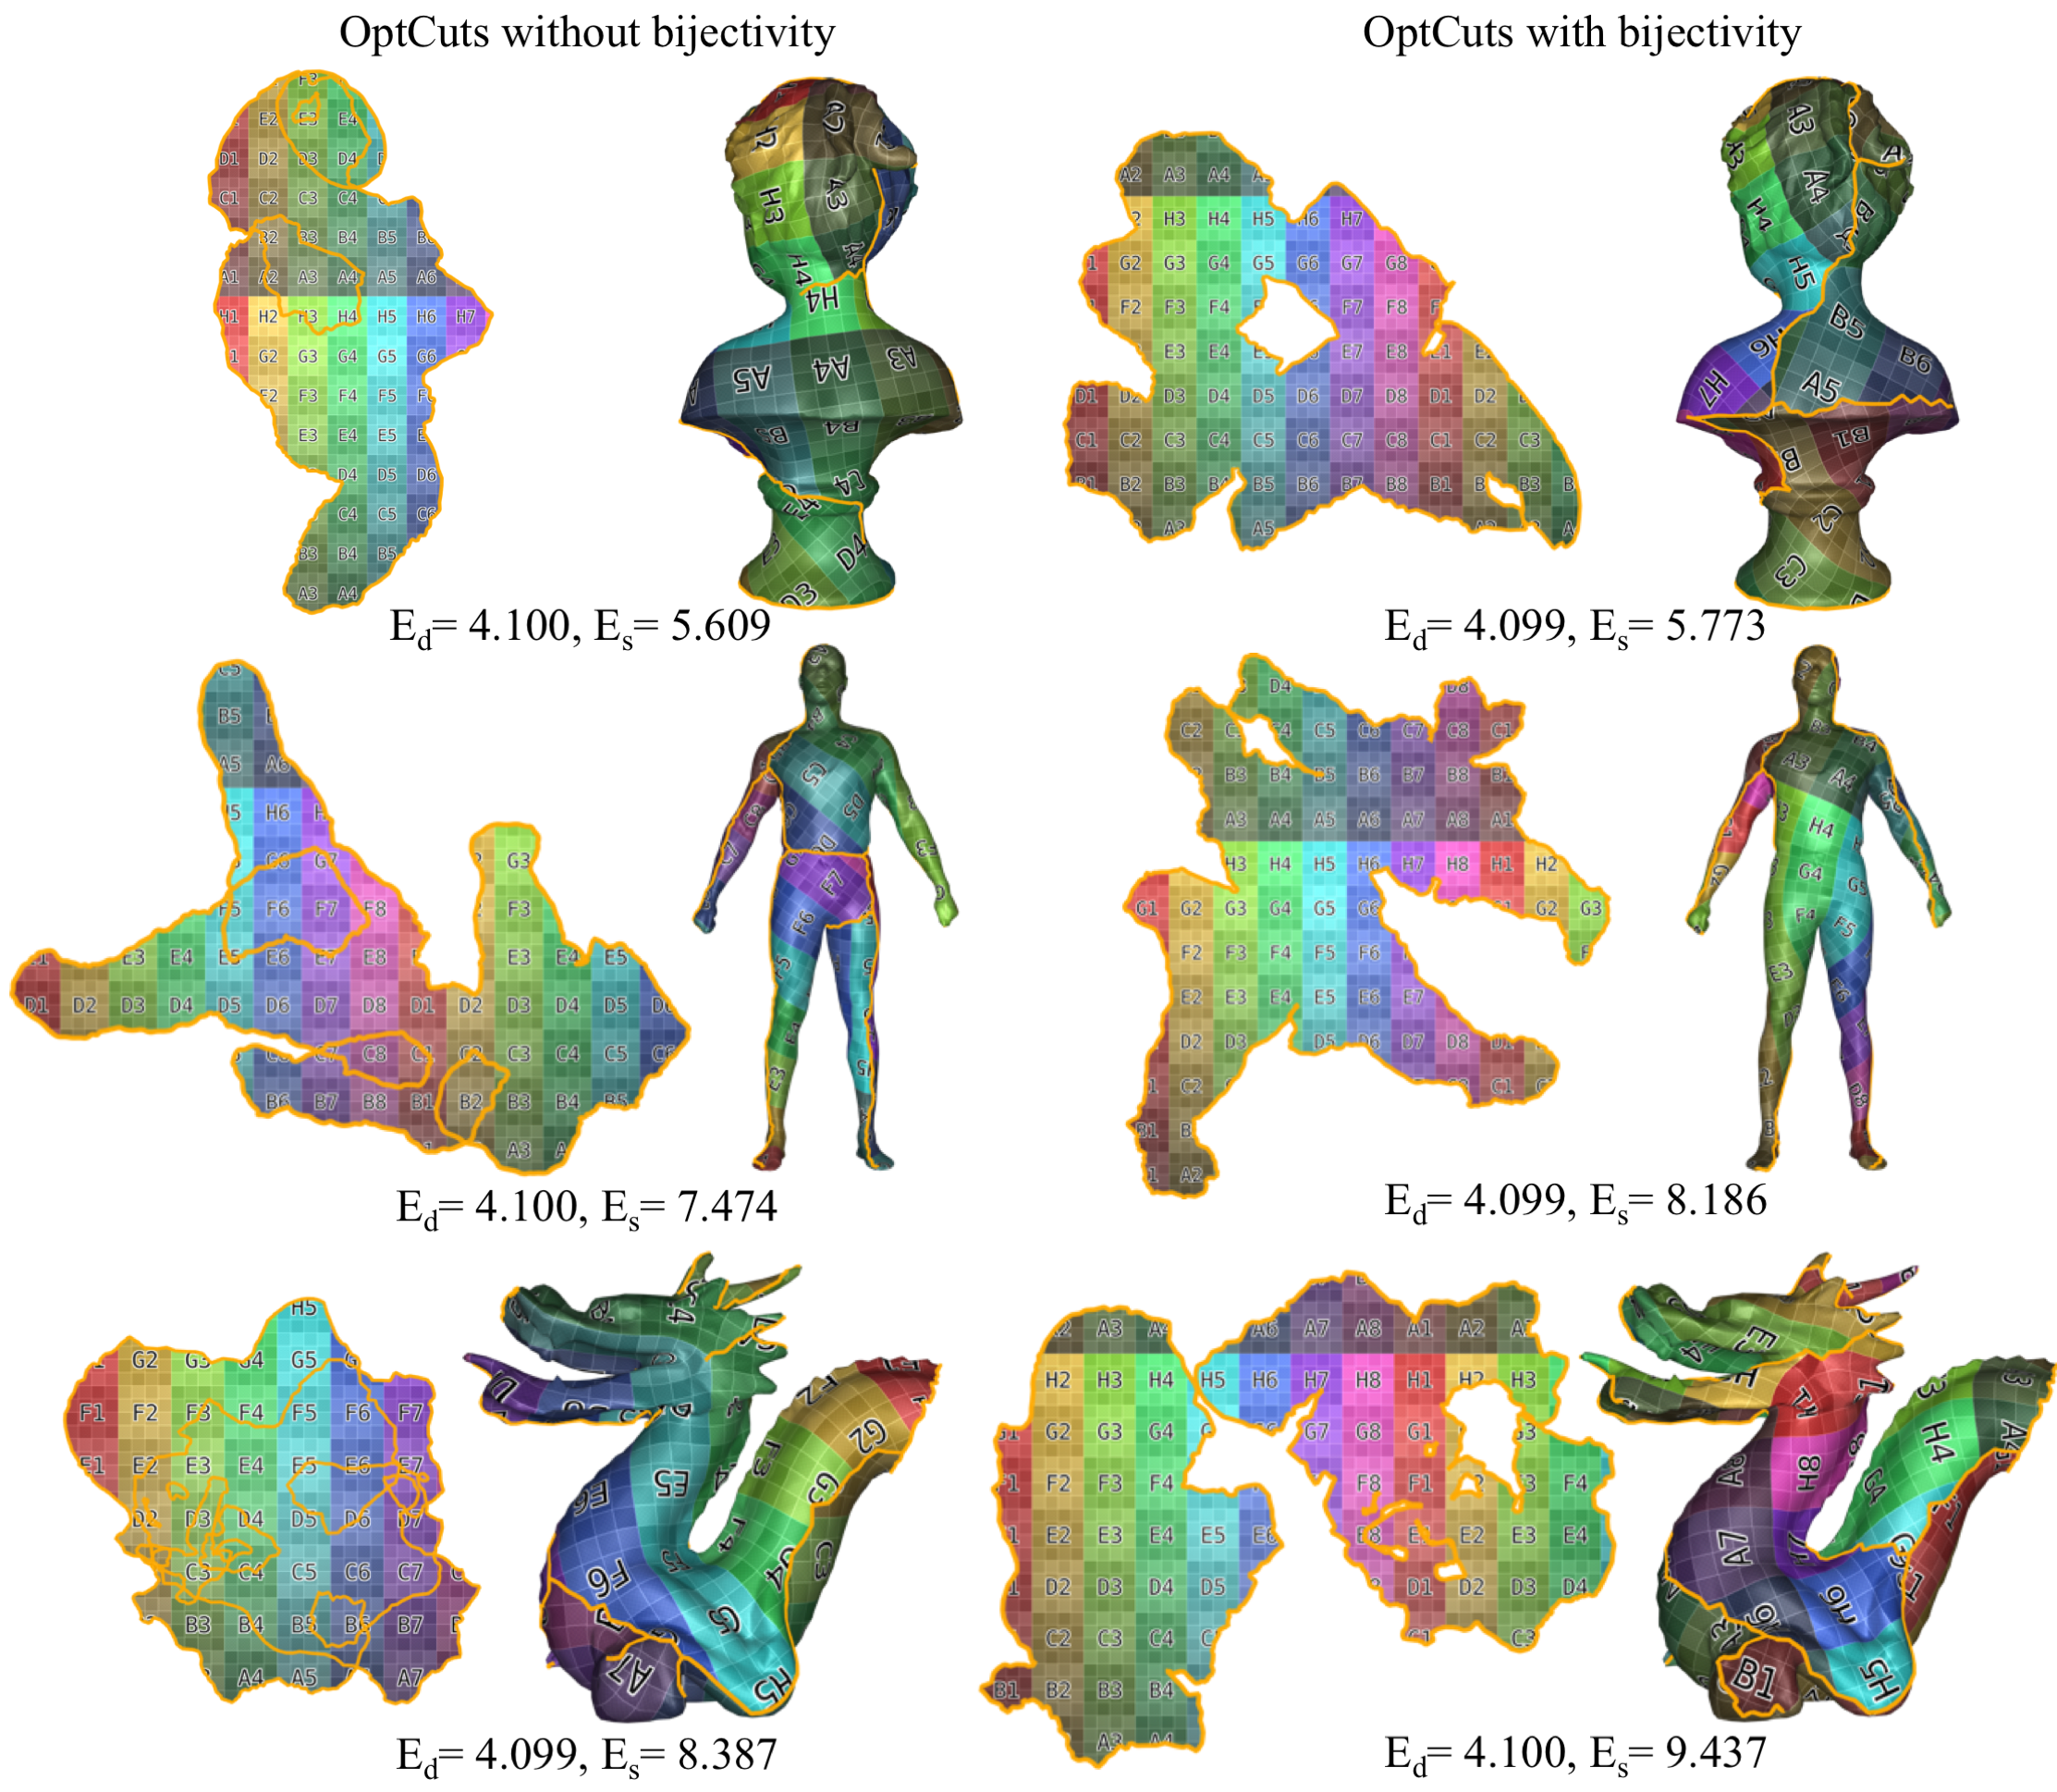
\includegraphics[width=0.5\linewidth]{fig/our_impressive_results_right.png}
\caption{UV maps generated by OptCuts with/without bijectivity with $b_d$ set to $4.2$, $4.1$, and $4.05$ from top to bottom.}
\label{fig:our_impressive_results}
\end{figure*}
%could also be bunny_i, statue_5, wooden_fish

\paragraph{Evaluation Metric}
We are able to directly use the output normalized $E_{s}$ as the evaluation metric since our method can generate UV maps with locally optimal seams under a certain distortion bound. This metric can be consistent among comparisons against all methods because given an input surface we are always able to compare the output $E_{s}$ under the same level of distortion. Moreover, it also fits in well with practical scenarios where the control of distortions are more intuitive to the users and as-short-as-possible seams are expected.

\paragraph{Initial Embedding}
\minchen{[TODO?]}
For closed surfaces, it is important to first obtain an initial seam for our method to construct the initial UV map. To show that we can always find a local optimum with respect to both the UV topology and coordinates regardless of initial embedding, we run our method on an input surface with several randomly picked initial seams and a heuristic initial seam that splits the shortest path between two farthest points on the surface. As demonstrated in Figure~\ref{fig:any_init_ends_well}, we produce high quality UV maps under the given distortion bound for all initializations.

\subsection{Comparison to AutoCuts}

We demonstrate the capabilities of our framework by comparing to the state-of-the-art AutoCuts~\cite{Poranne2017Autocuts}.
AutoCuts obtains high quality UV maps by involving users into the optimization loop. However, when aiming for convenient, fully-automatic methods, the non-smoothness of their Separation energy not only makes it challenging for global parameter settings, but also often end up the optimization with suboptimal results. To show that we automatically generate high quality UV maps without suffering from these issues, we compare our method with a fully automatic version of AutoCuts obtained under the guidance of AutoCuts authors by constructing appropriate homotopy paths with a uniform set of mesh-adaptive parameters. 
Specifically, we used $\lambda = 0.4$ and started with $\delta=100\overline{|e|}^2$ and half it in the beginning of each homotopy iteration until it reaches $10^{-4}\overline{|e|}^2$. Inside each homotopy iteration, we detect convergence by setting a tolerance $\sqrt{3n_t}\times10^{-3}\overline{|e|}$ on the $L^2$ norm of UV coordinate changes. Here $\overline{|e|}$ is the average edge length, $n_t$ is the number of triangles.

Since AutoCuts does not intuitively support generating UV maps with a certain level of distortion, we first run AutoCuts on a batch of input surfaces, and then set their output distortions as $b_d$ in our method for each input. As demonstrated in Table~\ref{tb:comp_AutoCuts}, for both the two versions of our method, we require less time to generate UV maps with same level of distortion but significantly smaller seams. Figure~\ref{fig:ESLBar_compAutoCuts} shows a bar chart comparison on the output $E_{s}$ of each input surface. Note that we easily enforced bijectivity (Figure~\ref{fig:comp_AutoCuts}), which is only supported in AutoCuts with user assistance on patch manipulation.

\begin{table}[!h]
\centering
\caption{Comparisons between AutoCuts and OptCuts with/without bijectivity (WB/NB) on 69 input surfaces with $3749$ vertices per input in average. Even with bijectivity, we achieve shorter seam length with less running time.}
\label{tb:comp_AutoCuts}
\begin{tabular}{|c|ccc|ccc|}
\hline
\multirow{2}{*}{method} & \multicolumn{3}{c|}{$E_{s}$} & \multicolumn{3}{c|}{time (s)} \\ \cline{2-7} 
                        & avg      & min     & max      & avg      & min    & max       \\ \hline
AutoCuts                & 7.5789   & 1.2069  & 24.6816  & 499.9    & 4.0    & 2677.0    \\
OptCuts(B)               & 5.8114   & 0.8979  & 19.7405  & 304.0    & 6.4    & 1267.7     \\
OptCuts               & 5.3065   & 0.8992  & 16.1329  & 148.7    & 3.1    & 650.9    \\ \hline
\end{tabular}
\end{table}

\begin{figure}[!h]
\centering
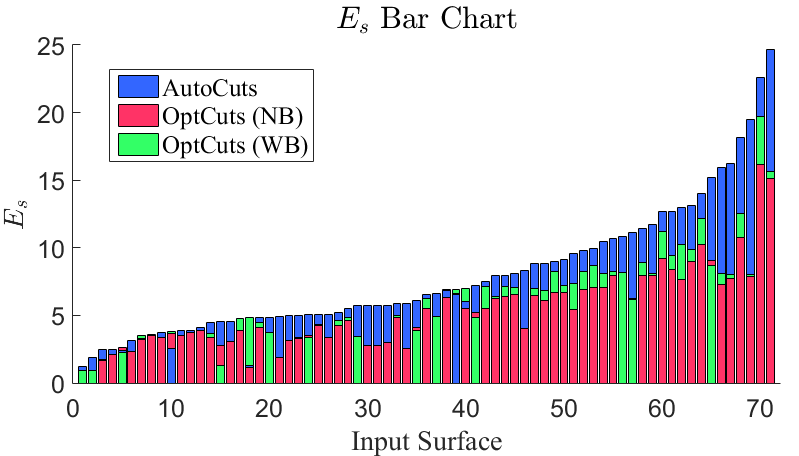
\includegraphics[width=\linewidth]{fig/ESLBar_compAutoCuts.png}
\caption{Normalized seam length $E_{s}$ bar chart of each example generated by AutoCuts and OptCuts with/without bijectivity. We achieve much shorter seams for almost all the inputs under the same levels of distortion.}
\label{fig:ESLBar_compAutoCuts}
\end{figure}

\begin{figure}[!h]
\centering
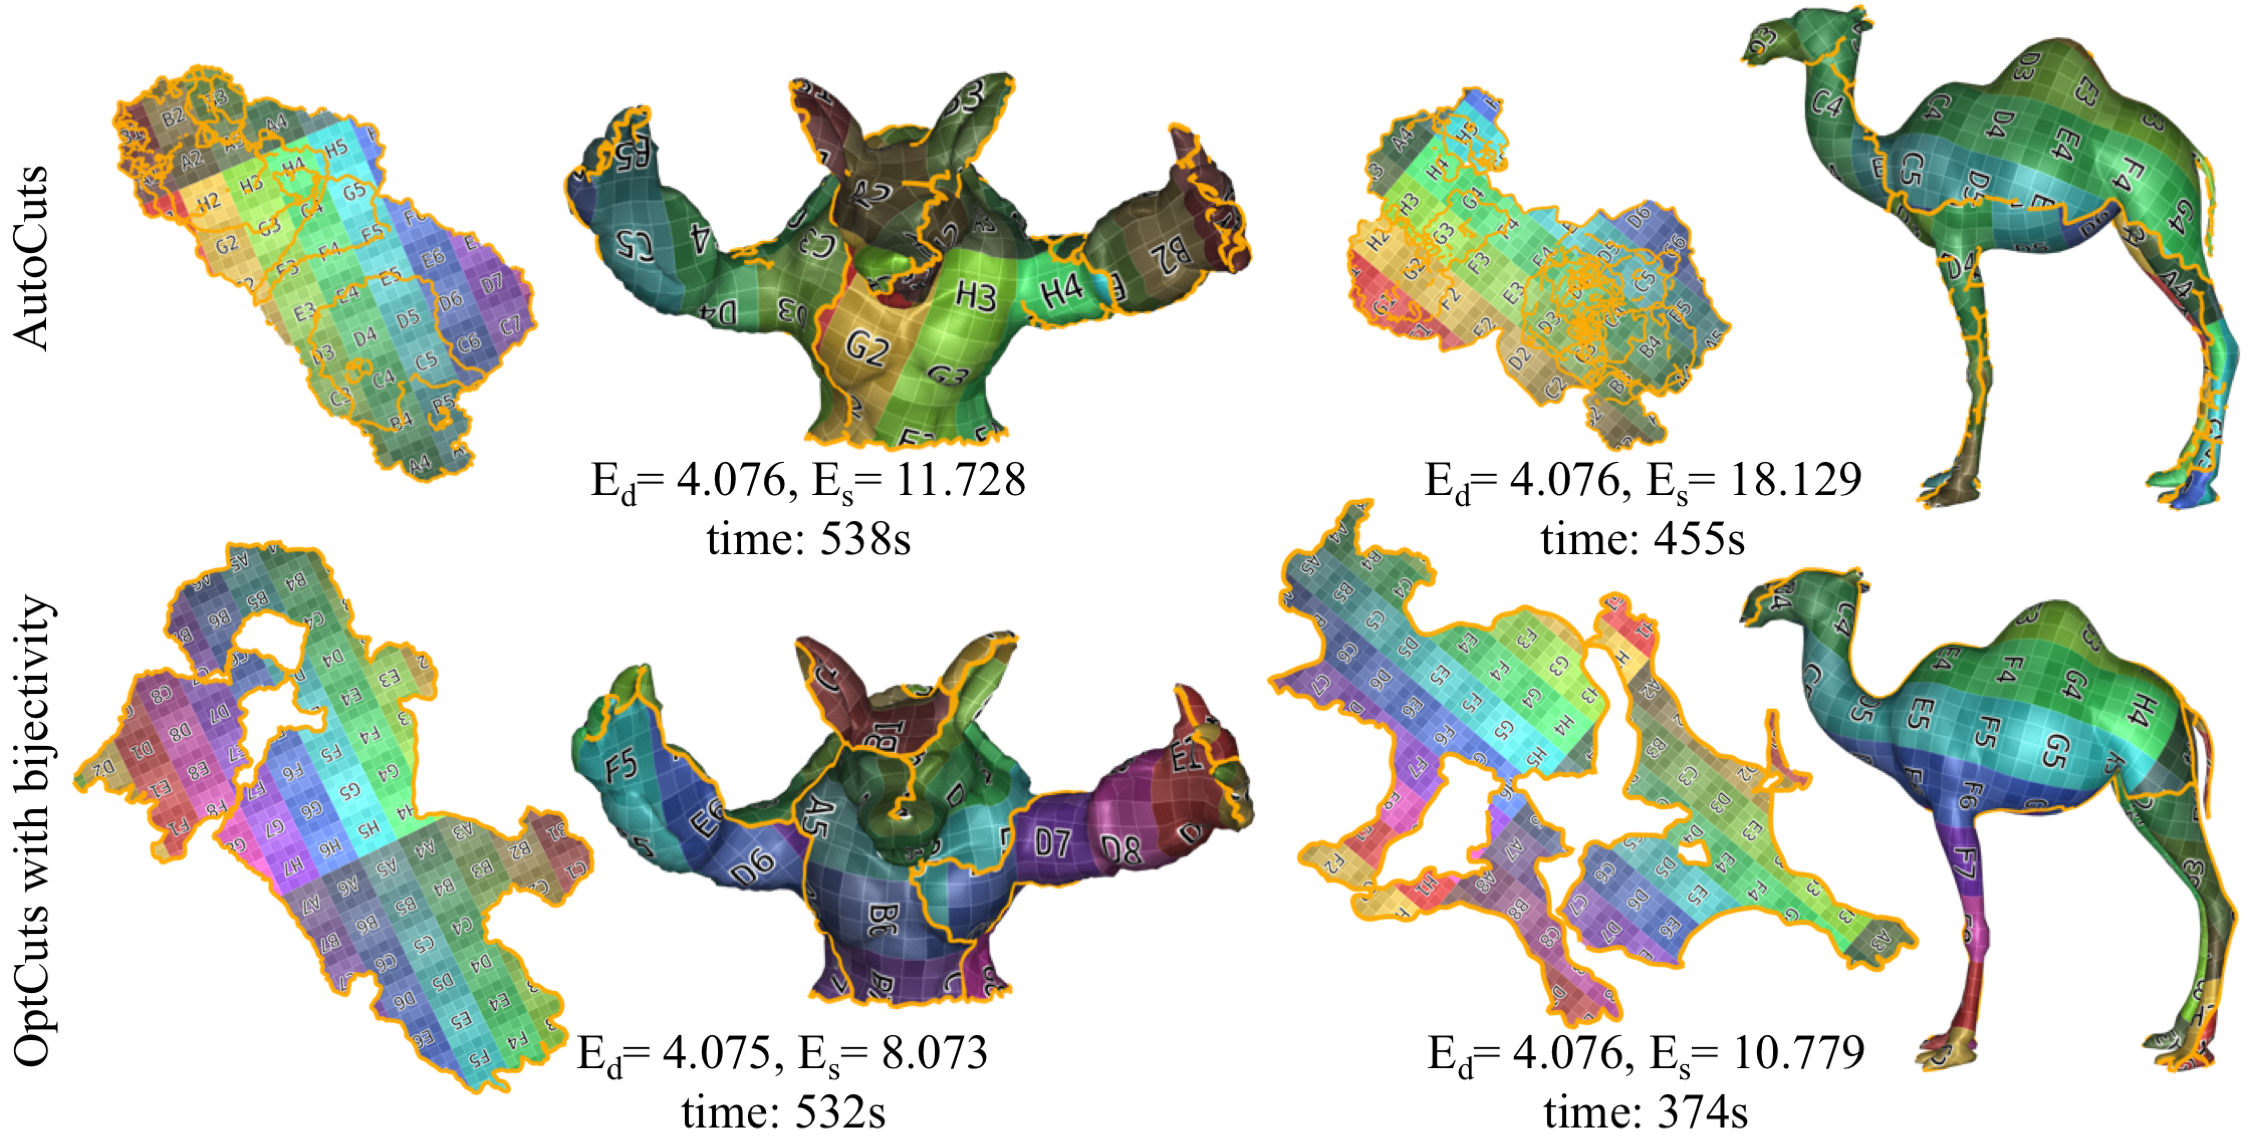
\includegraphics[width=\linewidth]{fig/comp_AutoCuts.png}
\caption{Comparison between AutoCuts (top) and OptCuts with bijectivity (bottom) on the armadillo (left) and camel (right) model, from which we can see that with a single set of parameters, AutoCuts may generate sub-optimal results for some inputs.}
\label{fig:comp_AutoCuts}
\end{figure}
% could also be bone_noInput, bunny_i_f10000, bunny, camel_vova_f10000, cat_noUV, cow_param_closed, dilo, horse, male_2, octopus, wooden_fish, foot_i_f10000, three_man_statue, gargoyle, rgb_dragon, statue_i_1, vase, venus

\paragraph{Scalability}
From the time-resolution scatter plot in Figure~\ref{fig:time_res_compAutoCuts}a, we see that for meshes with higher resolution, our method scales better on running time than AutoCuts.
We further run AutoCuts and our methods on 5 input surfaces obtained by progressively simplifying the original lucy model (48354 vertices) to test scalability. From the trend in Figure~\ref{fig:time_res_compAutoCuts}b, we further see that our method scales better. Besides, the average $E_{s}$ obtained by our methods with/without bijectivity on the lucy models are $9.236$ and $8.816$ respectively, much smaller than $13.052$ by AutoCuts. Notice that for models with 24200 and 48354 vertices, AutoCuts already run out of memory, since its system size is $6$ times that of ours.

\begin{figure}[!h]
\centering
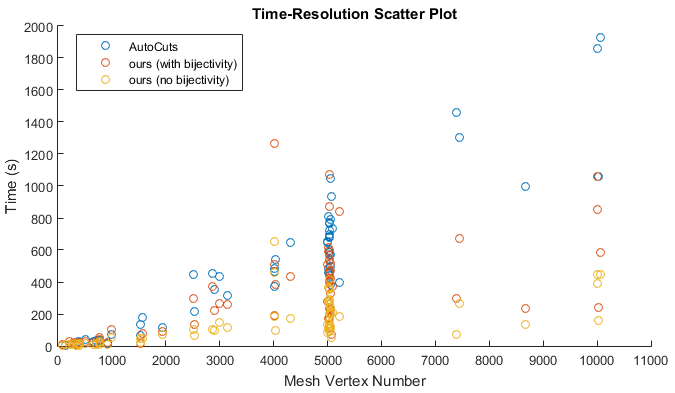
\includegraphics[width=\linewidth]{fig/time_res_compAutoCuts.png}
\caption{Time-resolution scatter plot of a batch of examples (a) and 5 lucy models with different resolutions (b) generated by AutoCuts and OptCuts with/without bijectivity. Note that in (b), there is no data points for AutoCuts on models with 24200 and 48354 vertices due to running out of memory. From the trend, we see that OptCuts scales better to meshes with higher resolution.}
\label{fig:time_res_compAutoCuts}
\end{figure}


\subsection{Variations}

\paragraph{Regional Seam Placement}
In texture painting applications, users would really like regions with the same semantic meanings stay connected or close to each other on the UV map. If we let users to select those regions on the input surface, we could easily avoid seams in those regions while still achieving bijectivity and similar seam length under the same distortion bound (Figure~\ref{fig:regional_seam_placement}). Without changing our framework, we just need to modify our formulation of $E_s$ by weighting each seam edge using the indicator function $w_{s}$ provided by the user:
\[ E_s = \hat{E}_{s} = \sum_{i\in\mathcal{S}} w_{s,i} E_{s,i} \quad w_{s,i} \in [1.0, +\infty] \]

\begin{figure}[!h]
\centering
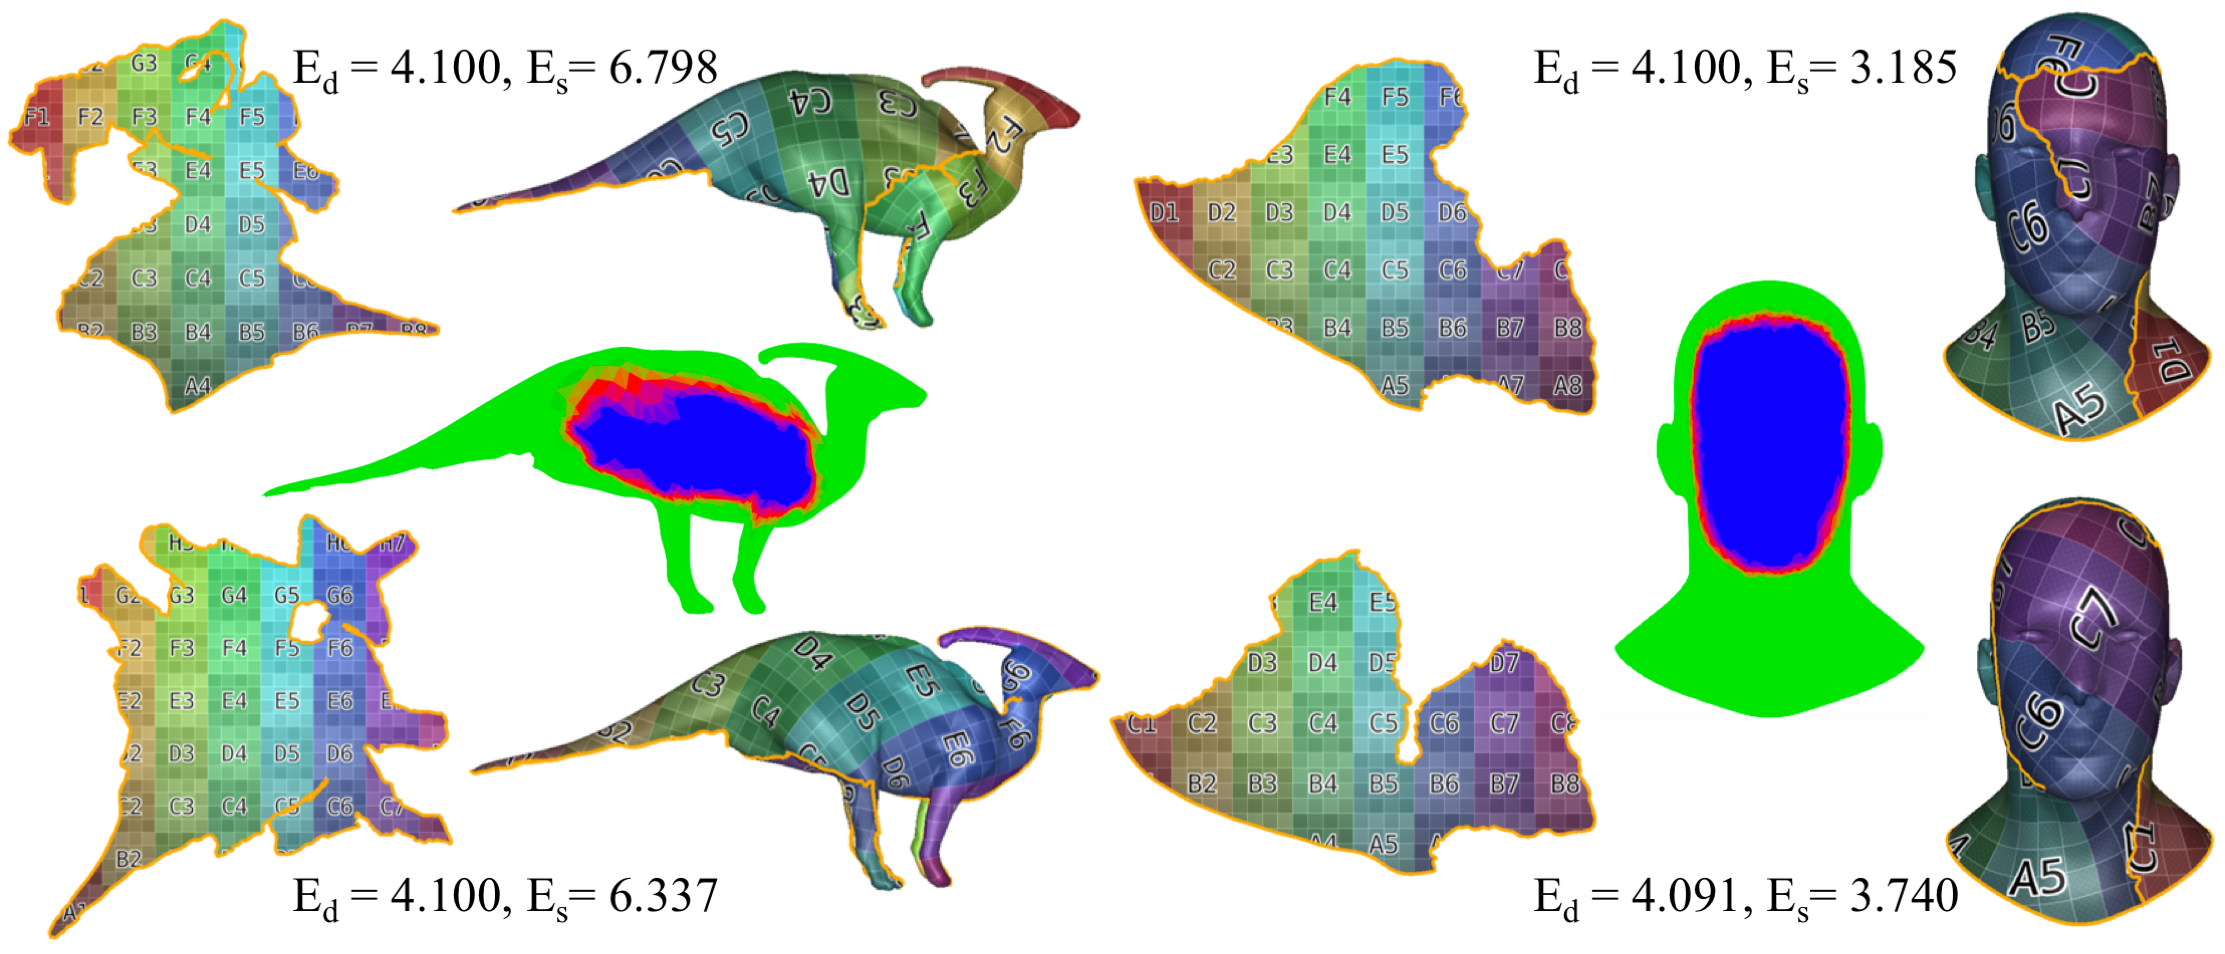
\includegraphics[width=\linewidth]{fig/regional_user.png}
\caption{Two examples of user controlled regional seam placement. Up to bottom: UV maps generated by the standard OptCuts with bijectivity and $b_d = 4.1$, user preference on regional seam placement (blue means seams are less wanted), UV maps generated by the variation of our method supporting the given user preference (with bijectivity and $b_d = 4.1$). For the left dilo model, we achieve shorter seam length with the regional constraints. This can also happen when involving our bijectivity constraints, since OptCuts is searching for local optimum.}
\label{fig:regional_seam_placement}
\end{figure}

% \paragraph{Conformal Parameterization}
% Using a conformal energy~\cite{Hormann2000MIPS,Sheffer2005ABFPP} for $E_d$ will achieve joint seam placement and conformal parameterization. Figure~\ref{fig:conformal_vs_isometry} shows some results with $E_d = E_{ABForMIPS}$~\cite{} compared to results with $E_d = E_{d}$, where different seams are generated while our framework stays the same.

\paragraph{Different Cutting Strategy}
The cutting strategy in the topology descent steps essentially build up the structure of the UV topology graph $\mathcal{G}_T$. By considering local topological operations, we built a dense graph connecting almost all the possible UV topologies and then reduce the search complexity by filtering. Alternatively, one can consider building $\mathcal{G}_T$ using only a sparse set of UV topologies and more aggressive topological operations, like the extremity-boundary (EB) cut applied in Geometry Images~\cite{Gu2002Geometry}.

We could alternatively apply EB strategy in our framework without bijectivity constraints by simply alternating the cut with distortion minimization processes, and stop right after $b_d$ is reached. This variation of our method reaches identical distortion bounds with very similar seam length compared to our standard method, but is much faster since the EB cut can be decided nearly instantly (Table~\ref{tb:comp_GI}). However, when we set smaller distortion bounds, the quality of the seams by EB cut drops since extremities are not that obvious on a nearly isometric UV map (Figure~\ref{fig:comp_GI}).

\begin{table}[!h]
\centering
\caption{Comparison between the standard OptCuts and using EB cutting strategy in our framework, both without bijectivity constraints. We run the two methods on 70 input surfaces with $3721$ vertices per input in average. With EB cutting strategy, we achieve similar seam length but much faster.} 
\label{tb:comp_GI}
\begin{tabular}{|c|c|ccc|ccc|}
\hline
\multirow{2}{*}{$b_d$} & \multirow{2}{*}{strategy} & \multicolumn{3}{c|}{$E_{se}$} & \multicolumn{3}{c|}{time (s)} \\ \cline{3-8} 
                       &                         & avg      & min     & max      & avg       & min    & max      \\ \hline
\multirow{2}{*}{4.2}   & OptCuts                    & 3.819   & 0.080  & 14.545  & 87.0   & 0.3 & 417.8 \\
                       & EB                & 3.868   & 0.159  & 14.929  & 13.0   & 0.1 & 72.1  \\ \hline
\multirow{2}{*}{4.1}   & OptCuts                    & 4.709   & 0.752  & 17.980  & 137.5  & 0.9 & 886.9 \\
                       & EB                & 4.795   & 1.207  & 16.895  & 17.0   & 0.1 & 87.2  \\ \hline
\multirow{2}{*}{4.05}  & OptCuts                    & 6.142   & 0.277  & 21.566  & 213.2  & 3.9 & 1398.1   \\
                       & EB                & 6.335   & 0.328  & 23.051  & 24.1   & 0.1 & 115.4 \\ \hline
\end{tabular}
\end{table}

\begin{figure}[!h]
\centering
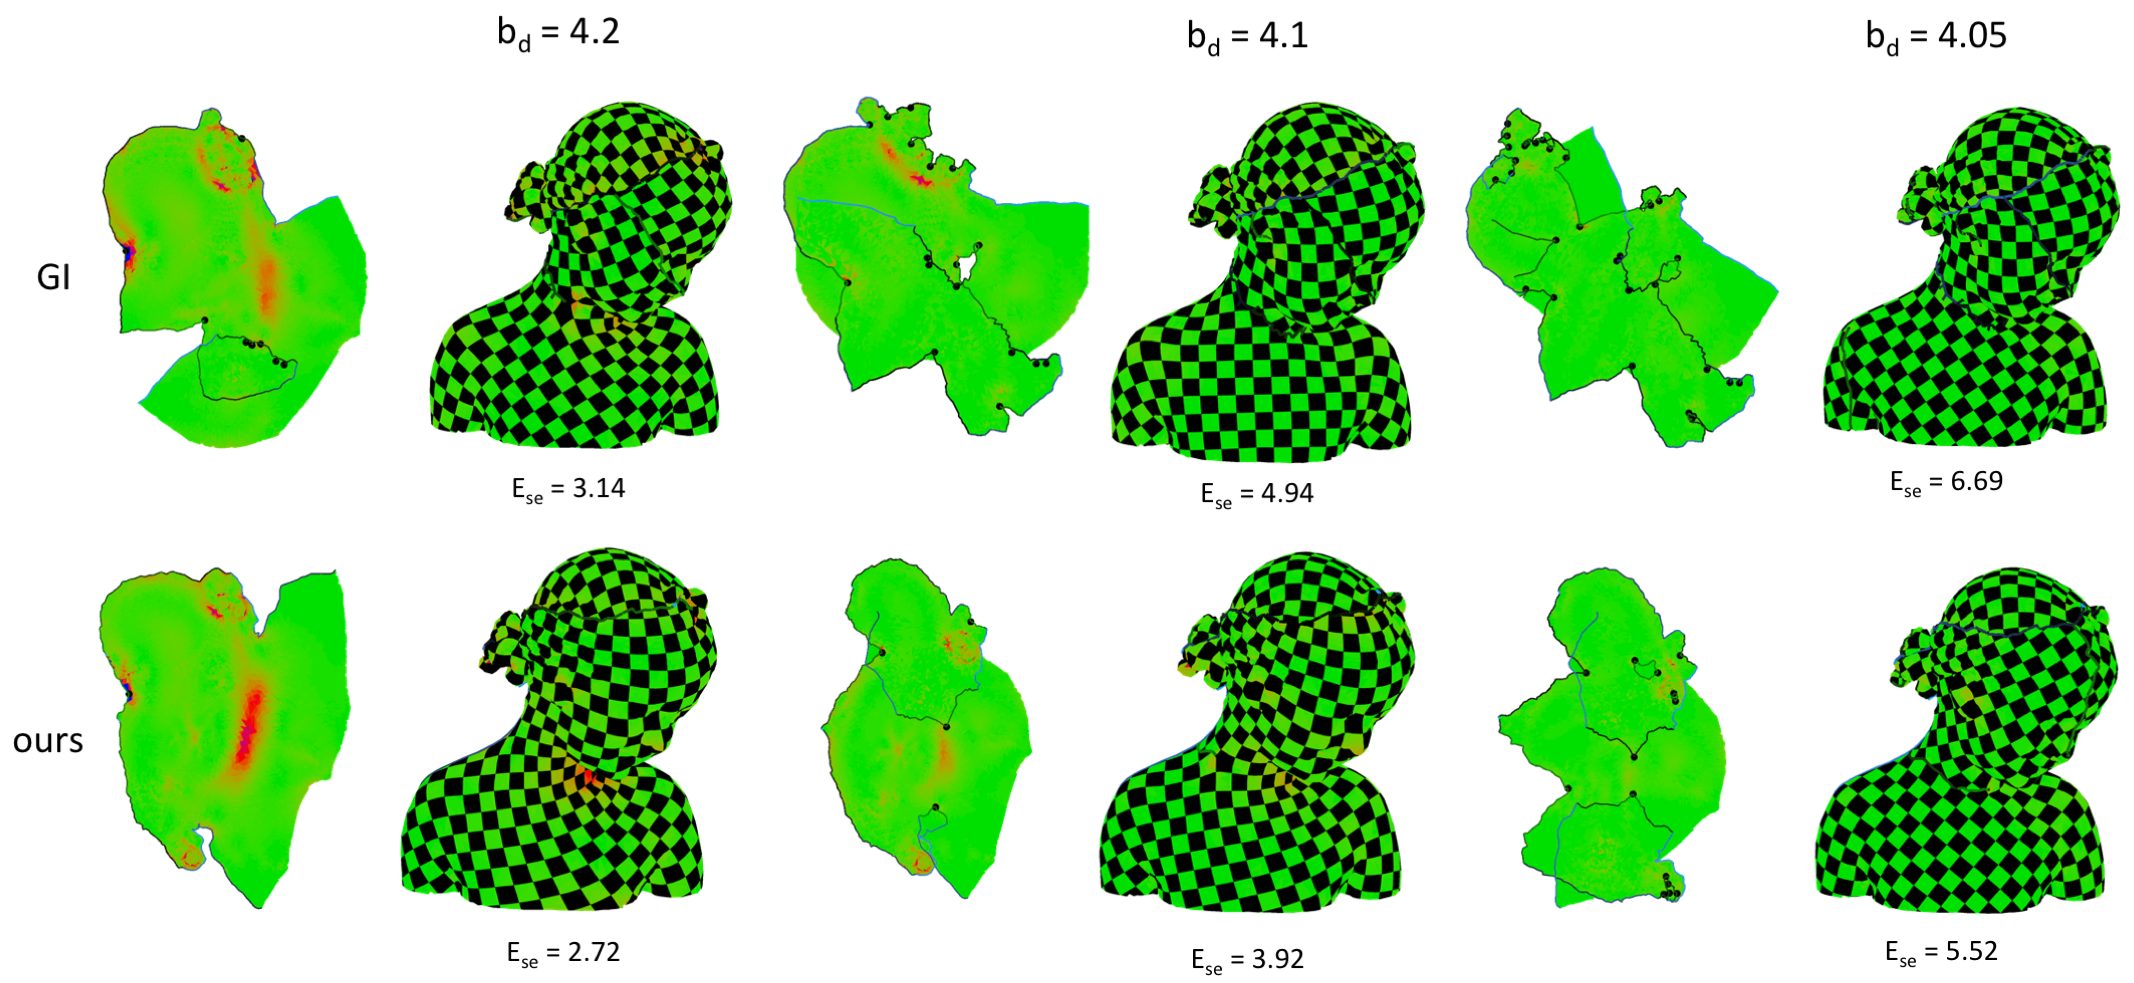
\includegraphics[width=0.8\linewidth]{fig/comp_GI.png}
\caption{Comparison between the standard OptCuts (left) and using EB cutting strategy in our framework (right), both without bijectivity constraints. EB cutting stategy is very efficient in early stages (a, b), but it does not work well when the UV map gets closer to isometric where extremities are not standing out (c).}
\label{fig:comp_GI}
\end{figure}
% also could be face_f10000, male_body_i_f10000, statue_4_i_f10000, statue_5_i_f10000, bimba_i_f10000

\paragraph{Warm Start}
Although we obtain high quality results given any initial embedding, the starting point does affect which local optimal point we will reach. Hence, it is meaningful to explore our method starting from initial seams with global observations. This will also benefit practical scenarios for improving preliminary UV maps while stay close to it.

If we take the output seams by our method with EB strategy to construct the initial embedding, we can improve the seam quality towards the nearby local optimal point while still satisfying the same distortion bound. Even if we add bijectivity constraints back, we still achieve shorter seam length compared to both our standard method without bijectivity and our method with EB strategy. (Figure~\ref{fig:comp_GI_outputAsInit}).

\begin{figure}[!h]
\centering
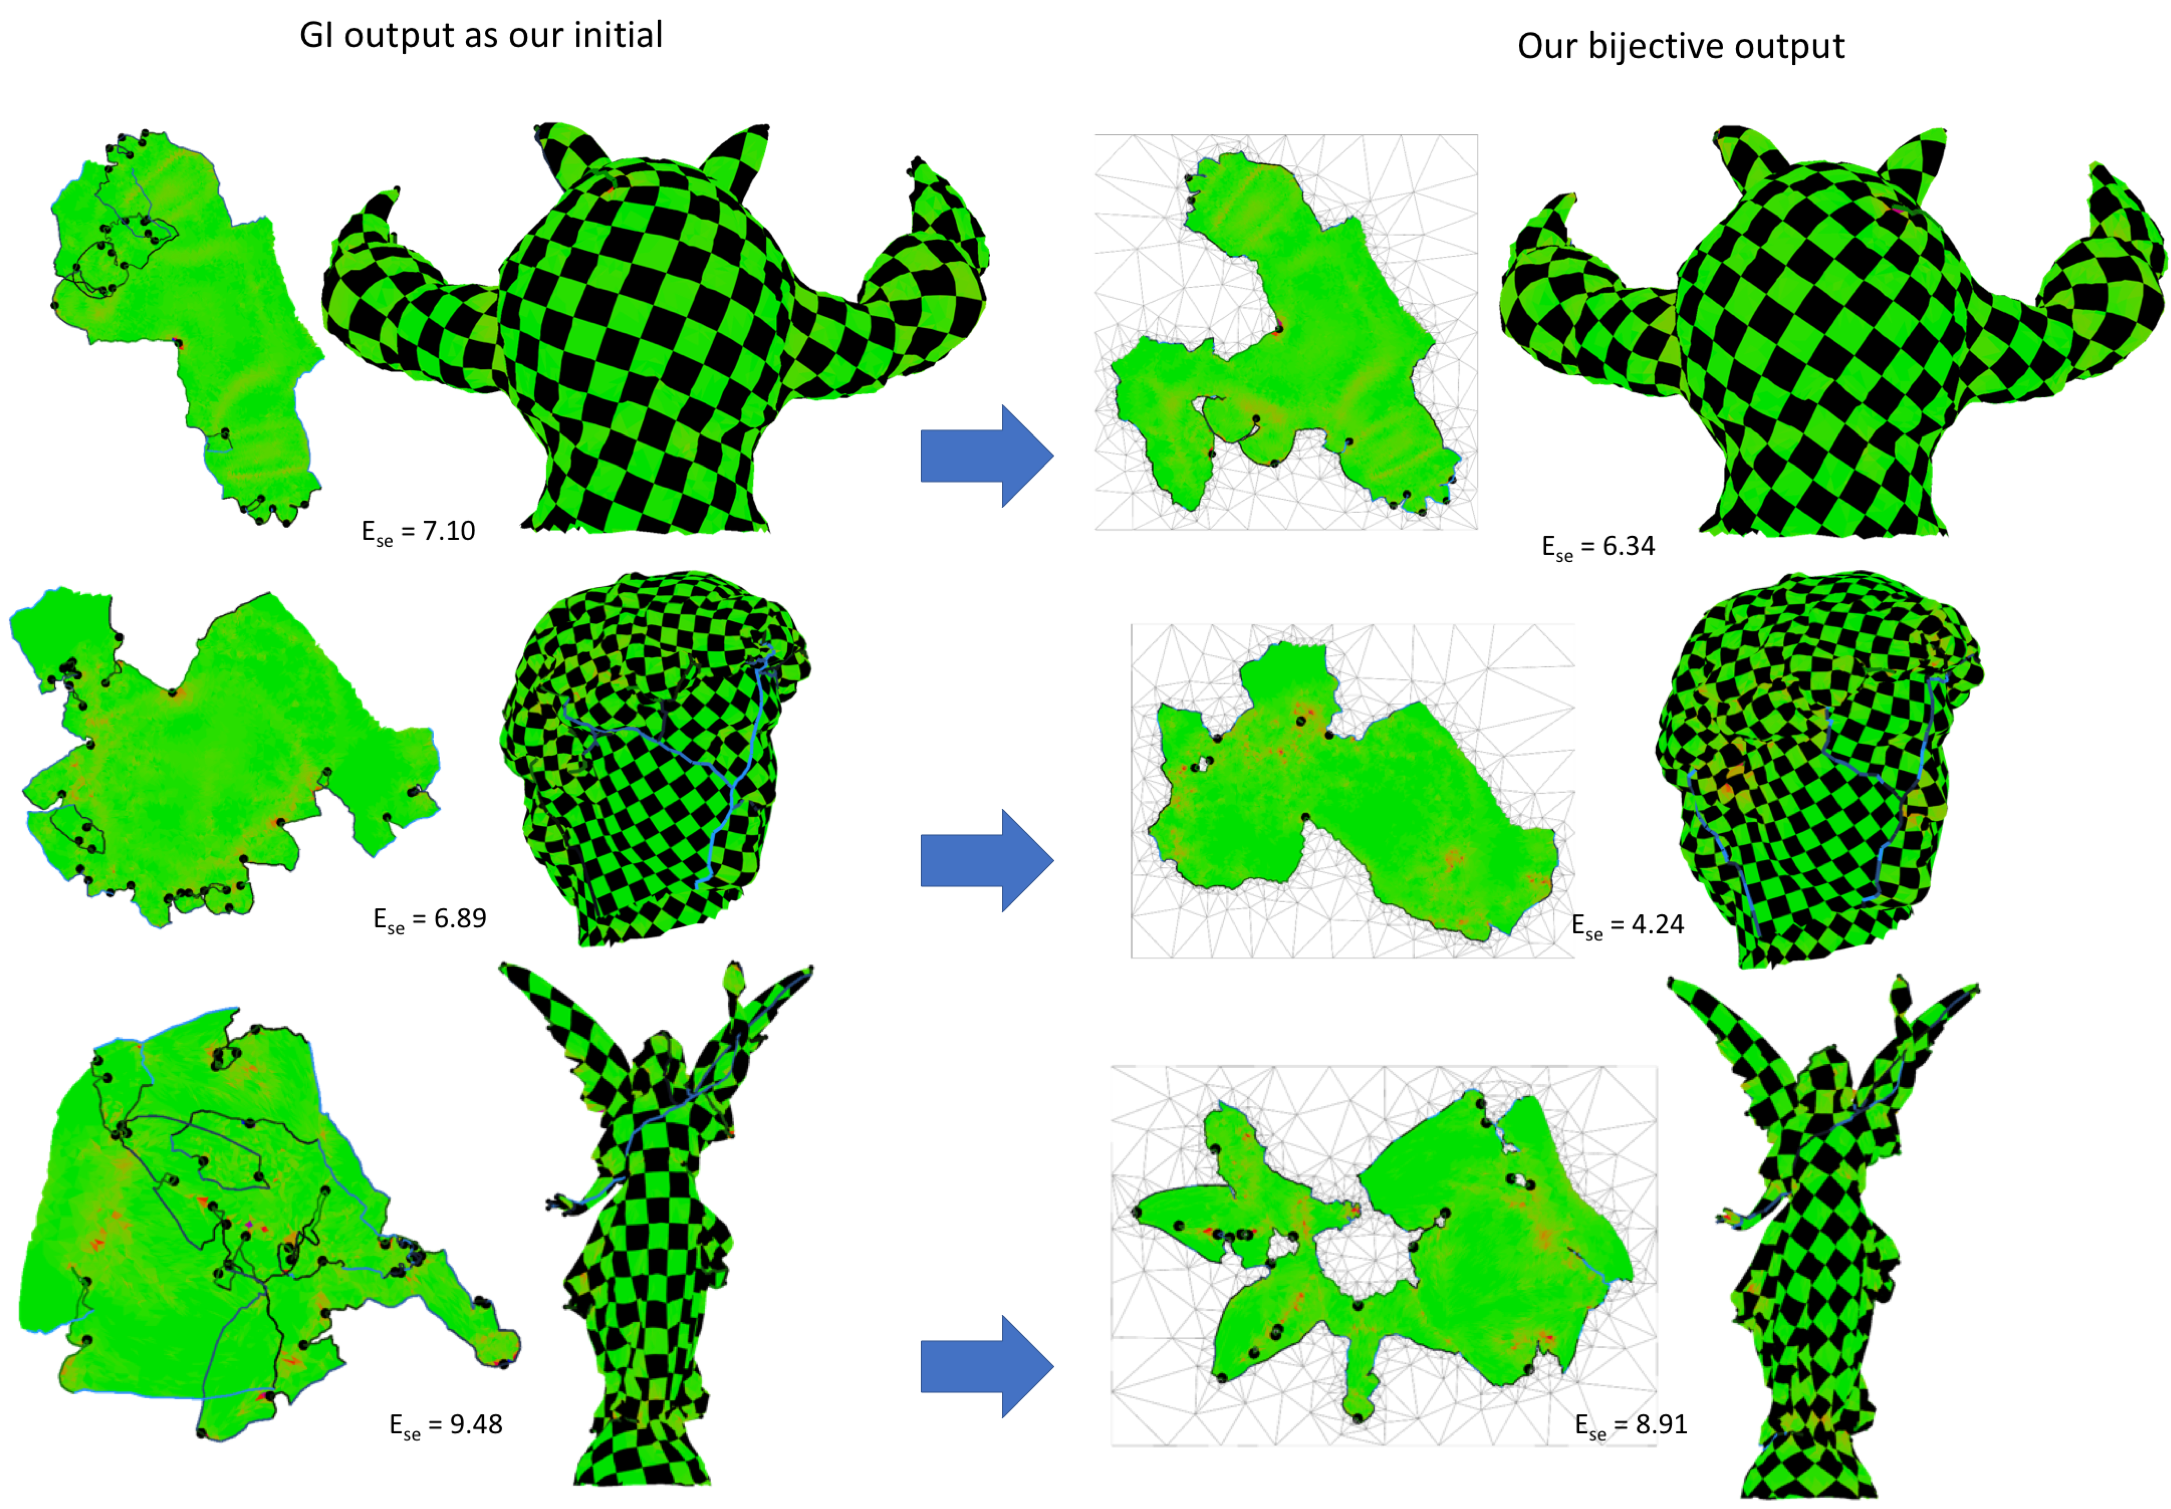
\includegraphics[width=\linewidth]{fig/comp_GI_outputAsInit.png}
\caption{Using output seams by our framework with extremity-boundary cutting strategy at $b_d = 4.1$ (a) as our initial UV map, we improve seam quality, reaching a locally optimal seam configuration under the given distortion bound even with bijectivity constraints (b). This seam length is also shorter than results obtained by standard OptCuts without bijectivity (c).}
\label{fig:comp_GI_outputAsInit}
\end{figure}
% also could be bimba, bunny

Seamster~\cite{Sheffer2002Seamster} is another classic seam cutting method worth considering for warm start. With Seamster's best output seams on the cow and triceraptop model, we obtain UV maps by minimizing $E_{d}$ with bijectivity constraints (Figure~\ref{fig:comp_Seamster}a), and use them for warm start, setting their distortions as the upper bounds. As demonstrated in Figure~\ref{fig:comp_Seamster}b, we achieve shorter seam length while maintaining the distortion bound and bijectivity. This seam length is also shorter than running our standard method without bijectivity from standard initialization (Figure~\ref{fig:comp_Seamster}c).

\begin{figure}[!h]
\centering
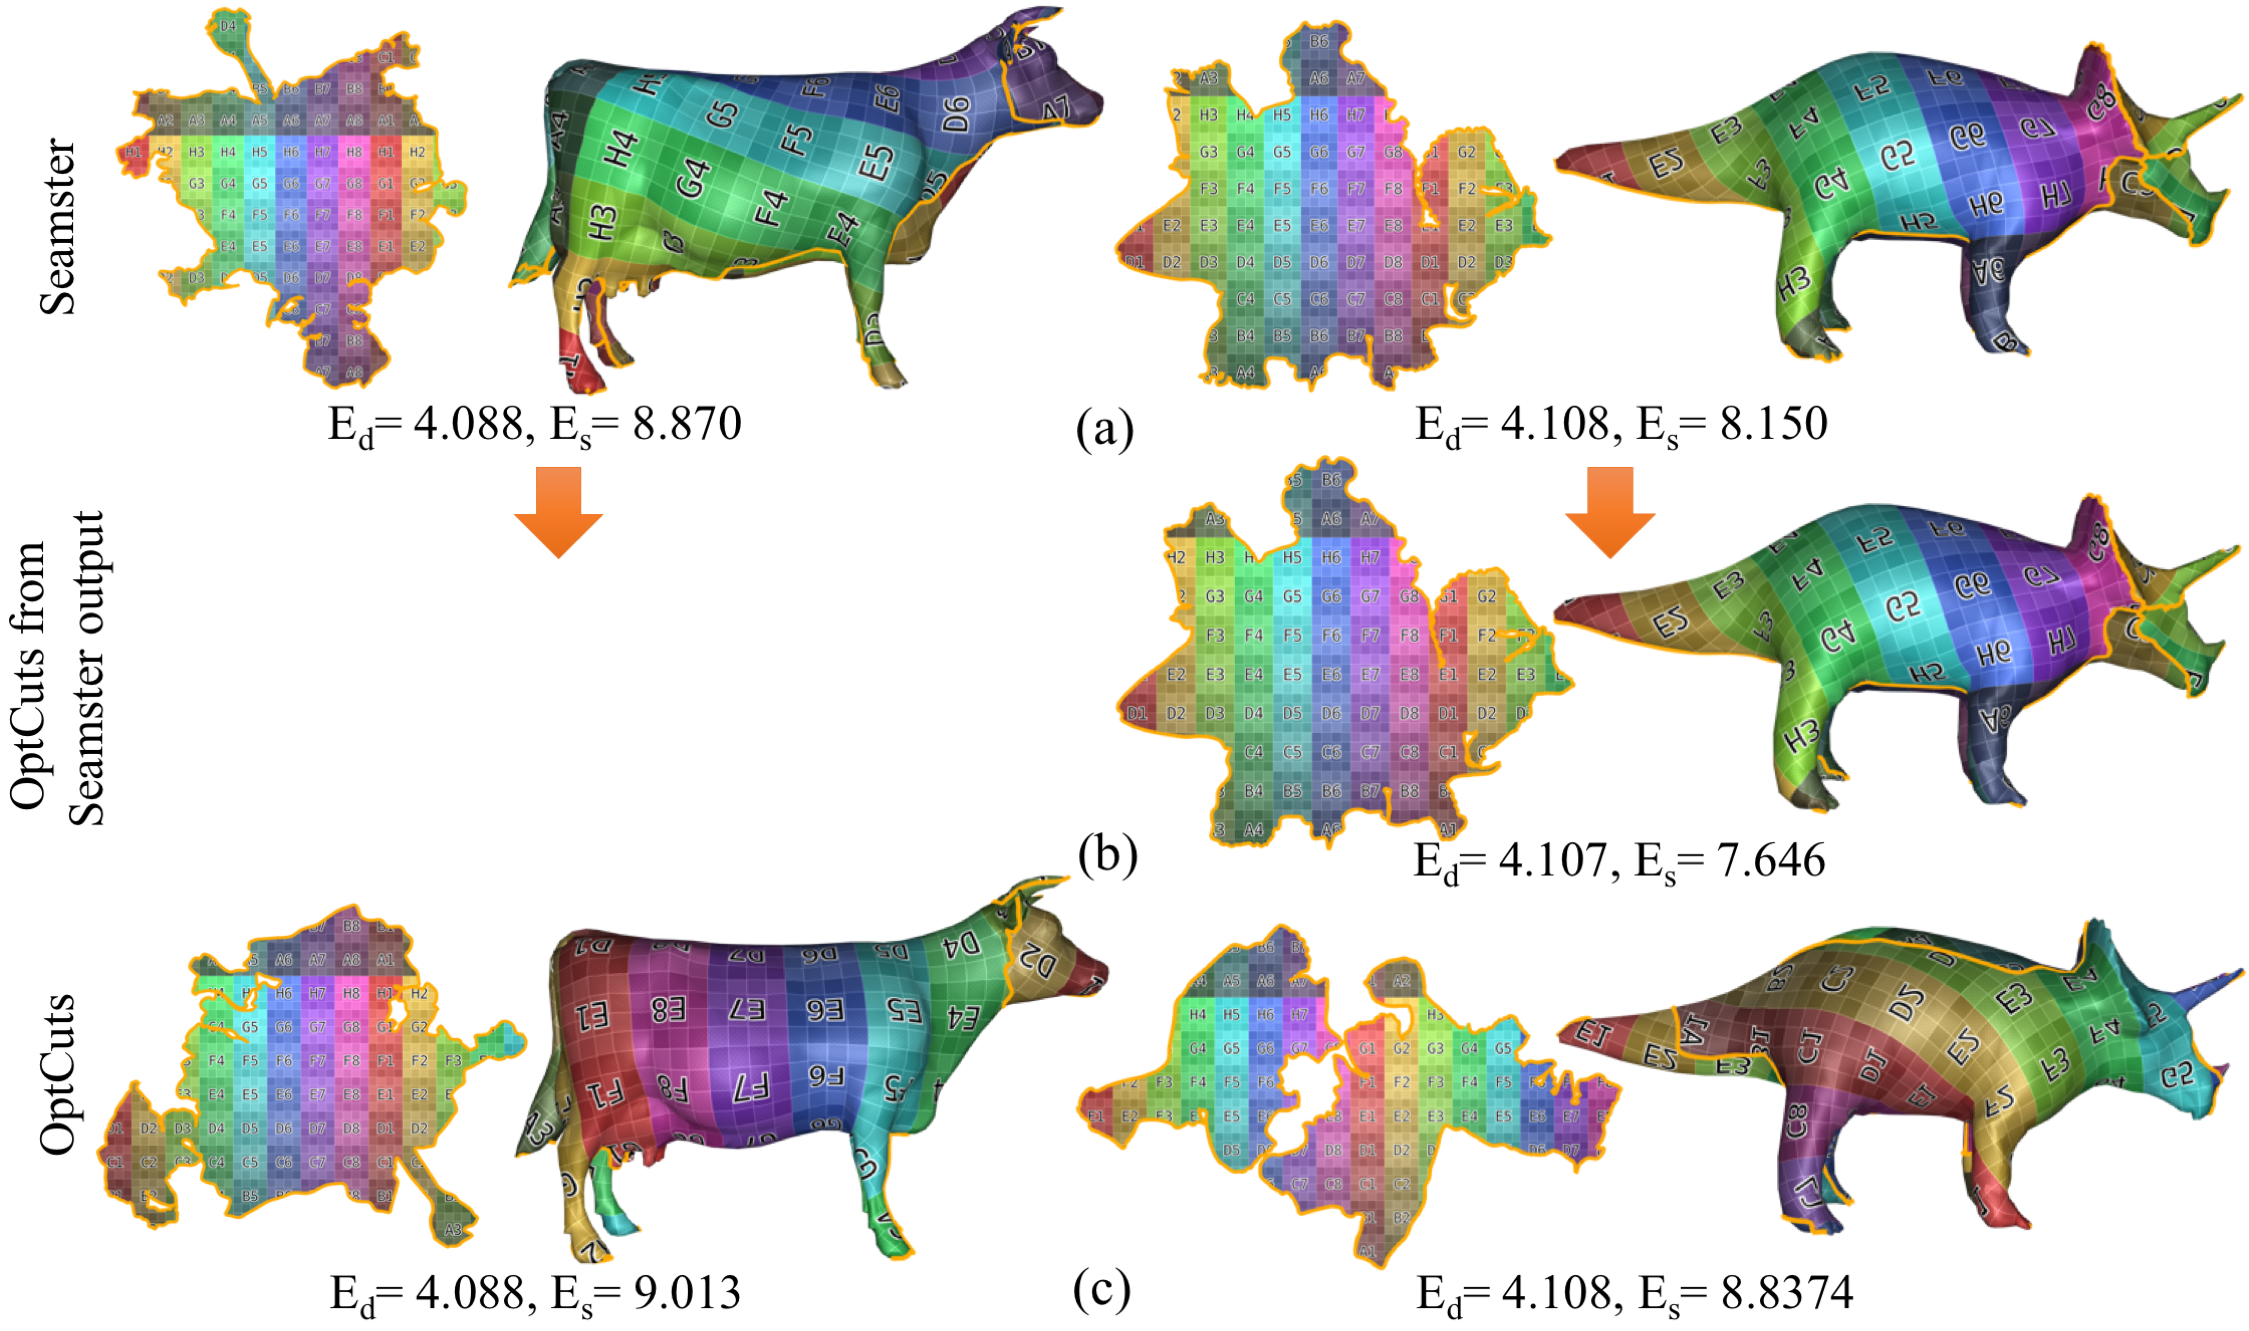
\includegraphics[width=\linewidth]{fig/comp_Seamster.png}
\caption{\minchen{[trouble stitching cow mesh together while maintaining the UV coordinates, will fix soon]} Starting from UV maps obtained by using Seamster's best output seams (a), we improve seam quality, reaching a locally optimal seam configuration while maintaining the distortion and bijectivity (b). This seam length is also shorter than running standard OptCuts without bijectivity from standard initialization (c).}
\label{fig:comp_Seamster}
\end{figure}

For Seamster, user need to set the size of local regions for measuring extremity, which is a mesh and shape dependent parameter that requires fine tuning. Even OptCuts with standard initialization achieves similar seam length without any user assistance.
